
%%%%%%%%%%%%%%%%%%%%%%%%%%%%%%%%%%%%%%%%%%%%%%%%%%%%%%
\section{Evaluation} \label{sec:evaluation}

This section describes the evaluation of Iroko using our testbed built on top of
Mininet simulator. The main goal is to compare the performance against the
existing centralized and decentralized techniques like Hedera~\cite{hedera} and
DCTCP~\cite{dctcp} respectively.

\subsection{Benchmark suite}

For evaluation purposes we are targeting a small scale data center of 16 hosts
and 20 switches with FatTree topology. We took measurements for Hedera, DCTCP,
ECMP and with Non-blocking switch on the same test setup. ECMP measurement is
considered as the base line. Non-blocking is a hypothetical single switch fully
connected setup and is considered as the theoretical maximum we are aiming to
achieve.

For traffic simulation, we are using the same traffic matrices used in
Hedera~\cite{hedera}. We took measurements for the variations of the following 3
traffic patterns:

\begin{enumerate} \item Stride$\left(i\right)$: A host with index $x$ sends to
the host with index $(x + i)mod(num hosts)$.  \item Staggered Prob $\left(EdgeP,
PodP\right)$: A host sends to another host in the same edge switch with
probability $EdgeP$, and to its same pod with probability $PodP$, and to the
rest of the network with probability $1-EdgeP - PodP$.  \item Random: A host
sends to any other host in the	network with uniform probability. We include
bijective mappings and ones where hotspots are present.  \end{enumerate}

Since we are primarily concerned about reducing the latency and packet drops
while keeping utilization at maximum, we measured bisection bandwidth and
    average queue length on switches. The experiments last for 60 seconds for
    each benchmark and we consider only the middle 40 seconds.

\subsection{Bisection Bandwidth}

\begin{figure*} 
	\centering 
	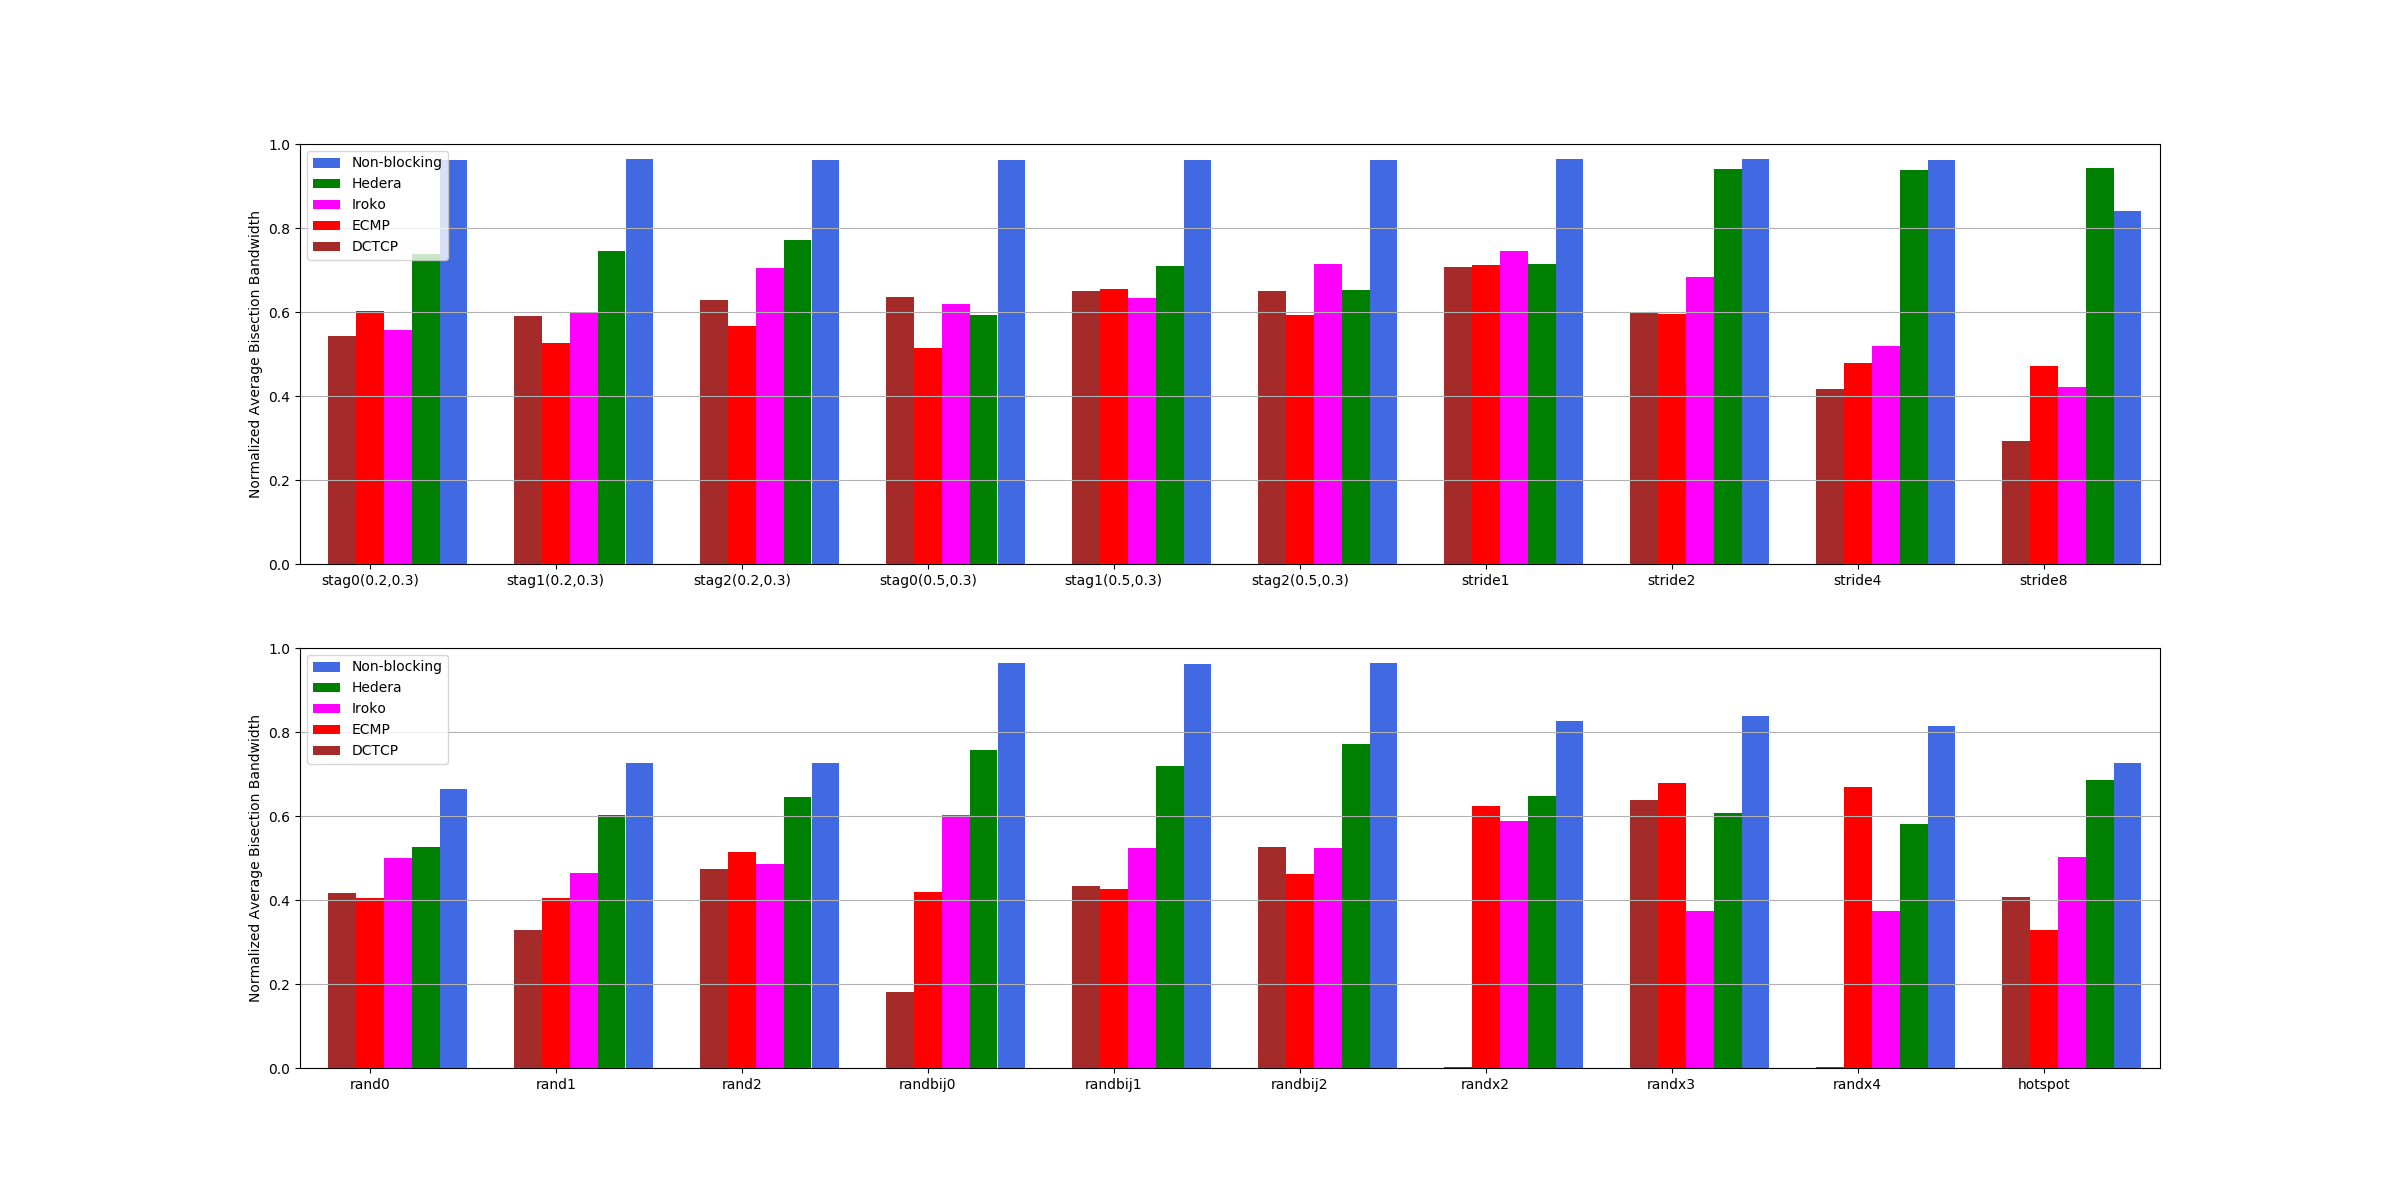
\includegraphics[width=1\linewidth]{rate.png} 
	\caption{}
	\label{fig:rate} 
\end{figure*}

In Figure \ref{fig:rate} we show the aggregate bisection bandwidth. Iroko
consistently provides better utilization compared to ECMP and DCTCP in almost
all experiments. As expected non-blocking is providing the best performance out
of all four techniques. Utilization of non-blocking is lower for traffic
patterns with high incast. Hedera perform extremely well in all experiments
except for some where Iroko outperforms Hedera. Interestingly enough, Hedera
even outperforms non-blocking limit in stride8 experiment. ECMP does reasonably
well when there is high probability of local communication for example smaller
strides, but start to deteriorate as the stride length increases because of hash
collisions.

Another interesting observation is that DCTCP gives abysmal utilization for some
experiments. Further investigation into this revealed that this is because of
DCTCP's aggressive congestion window size reduction strategy on incast. The
proposed solution for incast problem is to use dynamic buffer allocation in
switches which is not implemented in our test setup. General performance of
DCTCP is not satisfactory either. For some experiments it even under performs
ECMP.  According to DCTCP paper it is optimized for some specific data center
traffic patterns like web search, soft real-time applications, recommendation
systems etc which we don't include in our experiments.

\subsection{More Benchmarks}

Apart from utilization and loss rate following are the other benchmarks that we
are interested. We have not measured these yet due to time concerns.

\begin{enumerate}

\item \textbf{99th percentile latency:} Since we are aiming for a low latency
which means that 99th percentile latency in the network across all flows should
be as low as possible.

\item \textbf{Fairness:} Fairness across flows can be tested by introducing a
new host to a completely saturated network and increasing the transmission rate
to see if all the hosts gets fair share of the total bandwidth. Currently we are
assuming all flows should be at equal priority. Differential priority is out of
scope.

\item \textbf{Responsiveness:} This metric evaluates the predictive power and
efficiency of Iroko. It would be interesting to analyze the response time of the
central scheduler compared to decentralized DCTCP and TCP.

\item \textbf{Starvation:} Since we are rate limiting at the host level, Iroko
should make sure that no flows are starving to send data. This can be measured
by plotting residual bandwidth and excess load.

\end{enumerate}
